\section{Phrasing Additive Manufacturing as a Machine Learning Problem}\label{phrasing}

\subsection{The Assumptions Behind Machine Learning}
Ultimately, AM users desire a model that relates manufacturing parameters to AM material properties; i.e., a process-property model. In a functional form, this model can be written as
\eqn
f(x_1, x_2, ... , x_n) = \mathbf{y},
\label{fundamentalgoal}
\equ
where the inputs $x_i$ are $n$ different manufacturing parameters and the outputs $\mathbf{y}$ are measurable properties.

Currently, these process-property relationships are often developed by connecting separate process-structure and structure-property models of individual physical processes within AM.
For example, individual process-structure models are developed to relate : heat source parameters to melt pool topologies \cite{Khairallah2016} using the finite element method or similar computational techniques; melt pool topologies to solidification routes using thermal- and mass-diffusion models  \cite{Tan2011}; solidification to microstructure evolution using phase field methods \cite{Kundin2015}.
Separately, structure-property models are developed such as relating grain orientations and stress to material properties using crystal plasticity \cite{Pal2014}.
It is then by making connections between individual process-structure and structure-property models that researchers relate process parameters to material properties.
This understanding-through-sequential-modeling approach has the added detriment that the errors and uncertainty of each approach compound on one another, so that the final result is less accurate, more time consuming, and more expensive than the direct build-break approach to develop process-property relationships.
Machine learning is not a complete replacement for these traditional approaches, but rather a complementary modeling approach that can accelerate or even automate that process of building connections across many degrees of freedom that span the many different individual phenomenon within AM processes.
Two assumptions are necessary when using machine learning:
\begin{enumerate}
\item \textit{The Relational Hypothesis}: A correlative relationship exists between the data input to the model and the response of the system.
\item \textit{The Locality Hypothesis}: Parts manufactured at similar points in the design space will have similar properties.
\end{enumerate}

The first hypothesis is required for finding regression and classification functions that are physically accurate.

The second hypothesis is used to compare data and datasets, as well as to search and optimize through regression and classification algorithms.

\subsection{Unsupervised Machine Learning}\label{unsupervised}

Unsupervised machine learning algorithms are used to identify similarities or draw conclusions from unlabeled data by relying on the locality hypothesis.
Consider an experiment that varies three different manufacturing inputs $x_1, x_2, x_3$ and measures a single material property $y$.
In matrix form, the data are expressed as:

\eqn
\begin{split}
\mathbf{X} &= \begin{bmatrix}
	x_{1,1} & x_{2,1} & x_{3,1} \\
	x_{1,2} & x_{2,2} & x_{3,2} \\
	\vdots & \vdots & \vdots \\
	x_{1,m} & x_{2, m} & x_{3, m} \\
	\end{bmatrix} \\
\mathbf{Y} &= \begin{bmatrix}
	y_1 \\
	y_2 \\
	\vdots \\
	y_m \\
	\end{bmatrix} \\
\end{split}\label{initialmeasure}
\equ

where $x_{i,j}$ is the $j^{th}$ measurement of the $i^{th}$ manufacturing input.
A distance metric can be defined between data points in the design space.
For example, data can be collected at two points $\mathbf{a} = (x_{1}, x_{2}, x_{3})$ and $\mathbf{b} = (x_{1} + \delta, x_{2}, x_{3})$ and treat these quantities as vectors.
Computing the $\ell _2$ norm of $\mathbf{a}-\mathbf{b}$ yields

\eqn
|| \mathbf{a} - \mathbf{b}||_2 = \delta.
\equ





The value and magnitude of $\delta$ gives an inclination about how similar $\mathbf{a}$ and $\mathbf{b}$ are.
If $\delta$ is close to zero, then a researcher can say that they are similar, or even the same if $\delta$ is exactly zero.
As $\delta$ becomes larger a researcher can say $\mathbf{a}$ and $\mathbf{b}$ become more dissimilar.
The concept of `similar' manufacturing conditions may be easy to assess by an experimentalist when tuning only a few parameters at a time.
When taking into consideration tens or hundreds of design criteria, sometimes with correlated inputs, elucidating similar manufacturing conditions becomes difficult.
This vector distance approach is a simple, yet effective first glance at similarity in a design space and is generalizable to $n$ many design criteria.

Let us say that $\delta$ is small and that $\mathbf{a}$ and $\mathbf{b}$ are similar manufacturing conditions.
Now, consider a third point in the design space $\mathbf{c} = (x_{1} + \delta, x_2 + \delta, x_3)$ that has not yet been measured.
Since $\mathbf{c}$ was manufactured at similar conditions to $\mathbf{a}$, as measured by $||\mathbf{c} - \mathbf{a}||_2 = 2\delta$, then we may say that $\mathbf{a}$, $\mathbf{b}$, and $\mathbf{c}$ are all similar to each other. If the locality hypothesis is correct then manufacturing with conditions $\mathbf{a}$, $\mathbf{b}$ and $\mathbf{c}$ should yield similar measurements of $y$.

At some point, a researcher will have a set of initial manufacturing inputs $\mathbf{a}$, $\mathbf{b}$, $\mathbf{c}$, $\mathbf{d}$, etc., and associated property measurements that have been tested.
Churning through the remainder of all possible manufacturing conditions becomes expensive and tedious quickly.
Instead, researchers can use similarity metrics to determine whether or not a future test is worth running.
Comparing the manufacturing inputs through vector distance gives a rough idea of the possible outcome before spending time and resources on running a test.
If the intent is exploring design spaces then manufacturing at conditions \textit{furthest away} from previously observed points may be the answer.
If looking for local maxima of quality, an operator would want to manufacture at conditions \textit{nearest to} the conditions currently known to have high quality.

Using vector distances as metrics of similarities can produce results that are analogous to creating process maps \cite{Beuth2001}.
Process maps are used to divide $2$ dimensional plots of manufacturing inputs into regions of quality, or regions of different material responses.
The following demonstration is based on $k$-means clustering, a commonly used unsupervised machine learning clustering algorithm.

A researcher has acquired the datasets in Eqn. \ref{initialmeasure} and wants to partition $\mathbf{Y}$ into groupings of high quality parts and low quality parts.
However, there are several values of $y \in \mathbf{Y}$ that lie between two extremes and the cutoff for quality is not well defined.
It would be useful to use similarity metrics to find the best possible partition of quality.
To begin, the data set is partitioned randomly into two groups, $\mathbf{Y}_1$ and $\mathbf{Y}_2$.
The centroids $m_1$, $m_2$ (or centers of mass, in engineering) of each grouping can be calculated as

\eqn
	\begin{split}
		m_1 & = \frac{1}{|\mathbf{Y}_1|} \sum_{y_j \in \mathbf{Y}_1} y_j \\
		m_2 & = \frac{1}{|\mathbf{Y}_2|} \sum_{y_j \in \mathbf{Y}_2} y_j. \\
		\label{moment}
	\end{split}
\equ

where $|\mathbf{Y}|$ is the average value of a grouping.
The measurements were randomly partitioned at first; the goal is to re-partition each set so that similar measurements (similar levels of quality) are in the same set.
To do this, we can re-assign each set by

\eqn
	\begin{split}
		\mathbf{Y}_1 & = \{y_i : ||y_i - m_1||_2 \leq ||y_i - m_2||_2 \} \\
		\mathbf{Y}_2 & = \{y_j : ||y_j - m_2||_2 \leq ||y_j - m_1||_2 \}. \\
	\end{split}
	\label{reassign}
\equ

We can interpret the re-assignment in Eqn. \ref{reassign} physically: if a measurement initially assigned to set $\mathbf{Y}_1$ is closer in distance to $\mathbf{Y}_2$ then it is \textit{more similar} to the other set.
Thus, it is re-assigned.
Since the original partition was random it is likely that there are low quality parts mixed in with high quality parts - in other words, outliers exist in each partition.
Measuring the similarity of each data point to the mean of the groupings re-classifies these outliers into groupings that are more reflective of their quality.

Once re-assignment is complete the centroids in Eqn. \ref{moment} can be re-calculated and updated.
Then, data points are re-assigned once more based on how similar they are to the centroid of each partition.
If we have partitioned the input settings $(x_1, x_2, x_3)$ along with their corresponding measurements, then we have lists of input settings which are likely to give good/bad quality parts.
Further analysis can also be conducted, such as analyzing which regimes of inputs lead to good or bad quality - this is precisely what process maps represent.
The difference in this case is that $n$ many manufacturing conditions can be related to a quality metric simultaneously, with little to no human inspection or intervention.
Additionally, a researcher can dig further and analyze \textit{why} groups of input settings result in given quality for a material property.



\subsection{Supervised Machine Learning}
In a \textit{supervised machine learning algorithm} the goal is to find a relationship $T: \mathbf{X} \to \mathbf{Y}$ that best approximates the underlying physical relationship $f(\mathbf{x}) = \mathbf{y}$.
That is, supervised machine learning algorithms relate model inputs to labeled data.
It is not necessary to make any assumptions up front about the nature of $f(\mathbf{x}) = \mathbf{y}$ to find $T$.
We only need to rely on the relational hypothesis and assume the relationship exists.
The process of finding $T$ can take many forms, depending on the specific supervised ML algorithm being used.

One method to find $T$ is assume it is a vector that satisfies
\eqn
\mathbf{X}T = \mathbf{Y}.
\label{map}
\equ

A researcher usually seeks this relationship through the measurements they have observed; in this case, the measurements are stored in the matrices of Eqn. \ref{initialmeasure}.
A common method to find a vector representation of $T$, and a critical element in most machine learning algorithms, is through least squares regression. Least squares regression finds $T$ through a minimization problem, given by
\eqn
\min || \mathbf{X}T - \mathbf{Y} ||_{2}^{2}.
\label{leastsquares}
\equ
Equation \ref{leastsquares} can be interpreted analogously to similarity measurements for unsupervised algorithms: the closer that $\mathbf{X}T - \mathbf{Y}$ is to zero, the more similar $T$ is to $f(\mathbf{x})$.

%\textbf{This next example was specifically requested by a co-author for an explanation of how LSQ is done. I think it detracts from the conversation.}\newline

%In many cases the relationship in Eqn. \ref{map} is going to be over-determined (or \textit{rank deficient}) because a researcher will have more measurements than input parameters. There will be more rows of Eqn. \ref{initialmeasure} than columns. This means that a unique solution does not necessarily exist. $\mathbf{QR}$ decomposition is commonly employed to solve the rank deficiency of Eqn. \ref{map}. $\mathbf{QR}$ decomposition involves finding a representation of $\mathbf{X}$ as the product of two matrices, $\mathbf{Q}$ and $\mathbf{R}$. The columns of $\mathbf{Q}$ represent the basis vectors of the design space that $\mathbf{X}$ inhabits. $\mathbf{R}$ is an upper-triangular matrix whose entries are the coordinates of the data points contained in $\mathbf{X}$. This representation of $\mathbf{X}$ has two advantages. First, it decomposes the manufacturing inputs contained in the rows of $\mathbf{X}$ into basis vectors with coordinates, an easily interpretable representation. Second, the nature of $\mathbf{QR}$ decomposition ensures that $\mathbf{R}$ is a square matrix. Thus, any equation involving $\mathbf{R}$ will have exactly as many variables as it has unknowns, removing the over-determinedness of the problem \cite{Poole2011}.

%Using the $\mathbf{QR}$ decomposition transforms the problem stated in Eqn. \ref{map} into
%\eqn
%\mathbf{QR}T = \mathbf{y}
%\label{QR}
%\equ
%Since $\mathbf{Q}$ is orthogonal, and therefore invertible, we can now solve the problem
%\eqn
%\mathbf{R}T = \mathbf{Q^{-1}} \mathbf{y}.
%\equ

The method of solving equation \ref{leastsquares} are many and varied; indeed, much of this review will focus on applying Eqn. \ref{leastsquares} to various problems through additive manufacturing.
The result is an approximation to the functional relationship $f(\mathbf{x}) = \mathbf{y}$.
A new point of interest in the design space $\mathbf{x'}$ can be chosen and its associated material property $\mathbf{y'}$ can be predicted by computing

\eqn
\mathbf{x'}T = \mathbf{y'}.
\equ

This simple example demonstrates how functional relationships can elucidate more information about design spaces.
Commonly used machine learning algorithms in materials science and engineering are given in Table \ref{ML}.
Note that the field of Machine Learning is evolving as fast as AM itself; hence Table \ref{ML} is by no means a comprehensive review of all machine learning algorithms, but rather is intended to provide a comparison between the form and function of some of the most widely adopted algorithms in materials science and engineering.



%~_~_~_~_~_~_~_~_~_~_~_~_~_~_~_~_~_~_~_~_~_~_~_~_~_~_~_~_~_~_~_~_~_~_~_~_~_~_~_~_~_~_~_~_~_~_~_~
\subsection{Tools of the Trade}
Based on the previous discussion and examples, researchers are equipped with two general tools to integrate into ICME approaches, namely:

\begin{itemize}
	\item Measurement of similarity with distance metrics;
	\item Approximation of relationships $y=f(x)$.
\end{itemize}

These are the basic tools that will be used in the subsequent sections.
The method by which similarity is measured or $f(\cdot)$ is found is dependent upon the task at hand, the data being used, and the machine learning approach chosen.
In most cases, multiple appropriate approaches exist.

Throughout the rest of the article these two tools will be built upon and applied to a plethora of problems in AM.
In most cases, the discussion will be kept general - that is, the reader will be left to determine the best distance metric or regression tool to use.
In cases where specific methodologies already exist for a given problem the discussion will be more focused and exact.

\subsection{Design space considerations}
\label{subsec:DMC_design_space}
When attempting to optimize an AM workflow for a particular property, it is important to consider the size and complexity of the design space.
The size of this parameter space indicates the value of data-driven exploration.
While it may be most valuable to seed the design exploration by performing orthogonal experiments first(which could be determined using dimensionality reduction techniques), typical experimental conditions facilitate fine exploration of a small subset of the design space.
For example, a build plate of 44 samples is likely to be all of the same composition with each sample only differing by their part orientation on the build plate.
This hindrance suggests that seeding your design space from the currently available or past experiments will lead to desired output more quickly.

\begin{table*}
    \renewcommand{\arraystretch}{0.8}
    \setlength{\tabcolsep}{5pt}
    \begin{center}
        \begin{tabular}{@{}llll@{}}
            \toprule
            \hline
             Parameter & range & step size & levels \\ \midrule
            \hline
            \hline
            Skin/Contour/Core laser parameters: & & & \\
            Power & 100-200 W & 10 W & 10 \\
            Scan speed & 500-1000 mm/s & 100 mm/s & 5 \\
            Spot size & 50-100 $\mu$m & 10 $\mu$m & 5 \\
            Energy density & 1-5 J/mm$^2$ & 1 J/mm$^2$ & 5 \\
            \hline
            Build parameters: & & & \\
            Polar angle & 0-90$^\circ$ & 30$^\circ$  & 4 \\
            Azimuth angle & 0-180$^\circ$ & 90$^\circ$  & 3 \\
            Sieve count & 0-10 & 2 & 5 \\
            Amount of recycled powder & 0-100\% & 10\% & 10 \\
            \hline
            Other parameters: & & & \\
            Blade direction & 0-300 mm & 10 mm  & 30 \\
            Transverse direction & 0-300 mm & 10 mm  & 30 \\
            Hatch spacing & 0.1-0.50 mm & 0.1 nm  & 5 \\
            \hline
            \bottomrule
        \end{tabular}
        \caption{Typical AM design space set up for determining PSP relationships. Multiplying the factorial yields 10$^6$ possible experiments.}
        \label{table:design_space}
    \end{center}
\end{table*}

\subsection{Data pipeline}
\label{subsec:DMC_data}
There are a wide variety of computational tools associated with applying ML to materials science problems.
As there are not many large, robust, data sources for AM, developing a data pipeline should be a top priority for ML-focused AM teams.
Table\ref{table:data_tools} describes some common tools and how they may be useful to AM workflows.
It may be useful to breakdown the active learning process into four steps: identification, collection, condensation, and analysis.

\subsubsection{Identification}
Once an optimization goal has been set, it is useful to define the design space or number of experiments, that may be necessary to achieve such a goal.
A typical experimental design space may be dependent on two variables, the number of inputs and the level at which those inputs are varied.
For a typical build plate, it's possible to consider 10+ variables solely based on printing parameters.
Depending on the resolution to which each parameter should be varied, the design space will likely be too large to experimentally determine each value.
Table\ref{table:design_space}, illustrates potential parameters to consider for a typical AM design space.
While it is common to explore varying 2 to 3 of these parameters at a time, to fully explore this space would necessitate 10$^9$ experiments!

\subsubsection{Collection}
When optimizing a large design space, data collection may consist of two phases: uninformed collection and informed collection.
Initially, when no experiments have been performed, it is most useful to pick a subset of experiments that are most dissimilar to perform first.
In figure\ref{fig:SL}, due to the low dimensionality of the space, the most dissimilar experiments are easy to see.
For high-dimensionality design spaces, unsupervised learning techniques (t-SNE, PCA) may be useful to determine the most dissimilar experiments.

During both phases of data collection, it is useful to consider the number of format of initial data sources.
For AM, it is likely data will come from an instrument in the lab (i.e. XCT, mechanical testing) or previously recorded literature data.
When collecting data from literature tools like WebPlotDigitizer and Tabula are valuable for collecting data accurately and quickly.
Once data sources have been identified and some experiments have been performed it may be useful to unify disparate data into unique records.
For smaller projects, this could be as simple as transferring all relevant data to a csv.
For larger projects, users may want to consider an open data format, like JSON or SQL, to maintain robust data records.

\subsubsection{Condensation}
Condensing sparse data into an "ML-ready" dataset may vary greatly between projects but there are a few considerations specific to AM.
If multiple team members are collaborating on a project, it may be useful to consider standardizing input and output names ("Contour laser speed" vs. "Speed of contour laser").
This is important for both the research as it will ensure recorded properties are not incorrectly interpreted and for machine learning as unique strings are likely interpreted as different descriptors.
When working with large design spaces, Python packages like Numpy and Pandas do well to provide quick feedback for the density of a dataset and can highlight sparse areas of the design space.

During this phase, a resercher may also consider calculating features from raw data.
For example, the XCT may only record the size and position of pores but some pore statistics (min/max pore size) may prove useful for modeling.
During this step, the reseacher should apply their domain expertise to properly engineer useful features.

\subsubsection{Analysis}
Once some amount of a design space has been explored and the collected data has been condensed to the relevant properties of interest, machine learning algorithms may be able to guide which experiment to preform next.
Python packages like sklearn, tensorflow, keras, and OpenCV contain a variety of algorithms with well documented use cases.
For materials specific examples of implementing a sequential learning workflow, see the learn-citrination github respository.
Once an informative model has been generated, experiments should be optimized in batches that allow the model to improve over many cycles.
At this point, informed data collection, condensation, and analysis should be repeated until the design goal is realized.



\begin{table*}
    \renewcommand{\arraystretch}{0.8}
    \setlength{\tabcolsep}{5pt}
    \begin{center}
        \begin{tabular}{@{}llll@{}}
            \toprule
            Data source (instrument/software) & file type & processing tools & "ML-ready" output \\ \midrule
            \hline
            \hline
            X-Ray tomography (Zeiss Xradia Versa) & .tiff & image featurizer & vectorized image \\
            X-Ray tomography (TRACR) & .txt, .csv & Python (pypif, pandas, citriantion-client) & porosity statistics \\
            X-Ray diffraction (Panalytical empyrean) & .xy & Python (pypif, csv, pandas) & XRD features (\% desired phase) \\
            Optical microscopy (Keyence VHX-5000) & .tiff & image featurizer & vectorized image (grain size and distributions) \\
            Uniaxial tensile testing (MTS 370) & .xy & Python (Hough transform algorithm) & real-valued mechanical properties \\
            Composition (TOF-SIMS) & & Python (pymatgen, matminer, magpie) & composition feature vectors \\
            Semi-structured web page & .html & Python (requests, beautifulsoup) & csv-formatted records \\
            Semi-structured pdf (txt-based) & .pdf & tabula, AbbyyFineReader, Python (pdftotext) & csv-formatted records \\
            ML packages & & Python (sklearn, tensorflow, keras, OpenCV) & \\
            \hline
            \bottomrule
        \end{tabular}
        \caption{Common tools and packages for preparing data for ML applications}
        \label{table:data_tools}
    \end{center}
\end{table*}


\subsection{Preparing data for machine learning}

For materials synthesis applications, signal from machine learning models is often limited by the amount of data and the speed at which data can be collected.
Many standard algorithms are suitable to correlate high-dimensional inputs and outputs in the AM design space.

To prepare experimentally generated data for input to a machine learning model, python scripting and other automation tools are typically employed.
For AM synthesis optimization, data is generated at many disparate sources.
For example, after a build plate is printed, the porosity of each sample is determined through X-ray tomography while other mechanical properties are determined through tensile testing.
Data collected this way is typically resolved through a master record in which data from many instruments and synthesis steps is stored.
Also, storing these data in a human and machine-readable format allows for quick error checking and data maniuplation to be performed while still being accessible for machine learning.
Table XX highlights a variety of computational tools and Python packages and their relevance to AM synthesis optimization.


%\begin{figure}
%  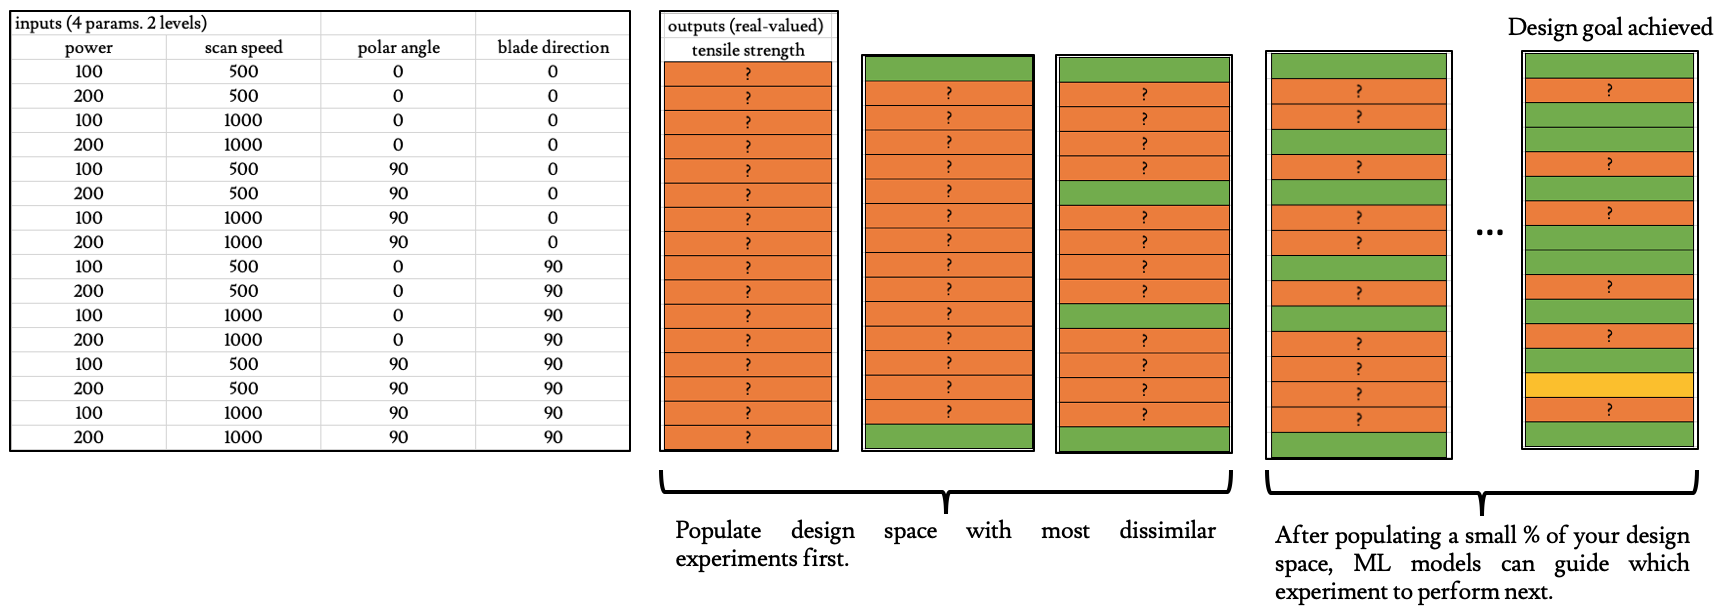
\includegraphics[width=0.9\linewidth]{SectionII/design_example.png}
%  \caption{Illustrating a sequential learning workflow. In this example, there are 16 total possible experiments and
%   4 experiments are performed for initial data collection. To reduce potential bias due subsampling of the input space,
%  the most dissimilar experiments should be performed first. After populating some amount of the design space,
%  machine learning should be used to begin informative data collection until design goal is realized.}
%  \label{fig:SL}
%\end{figure}

%%%
\begin{table*}[t]
\caption{Several of the most widely used machine learning algorithms that have been used in materials science are compared.} \label{ML}
\begin{tabular}{p{2.25cm}|p{2.25cm}|p{3cm}|p{4cm}|p{4cm}}
\raggedright Class of Algorithm & Examples & Applications & Strengths & Constraints \\ \hline \hline
Weighted neighborhood clustering & Decision trees, k-Nearest neighbor & \raggedright Regression, Classification, Clustering and similarity & These algorithms are robust against uncertainty in data sets and can provide intuitive relationships between inputs and outputs. See Ref. \cite{Quinlan1986} for a primer on clustering. & They can be susceptible to classification bias toward descriptors with more data entries than others. \\ \hline

\raggedright Nonlinear dimensionality reduction & \raggedright t-SNE, Kernel ridge regression, Multidimensional metric scaling &\raggedright  Dimensionality reduction, Clustering and similarity, Input/output visualization, Descriptor analysis, Regression, Predictive modeling &\raggedright These algorithms are robust against nonlinear input/output relationships and can provide intuitive projections of the material input/output space. For accessible examples, see Refs. \cite{Tenenbaum2000, Roweis2000}. & Projections can represent unphysical, difficult to interpret relationships. Global relationships can also be lost when nonlinear dimensionality reduction results are projected onto lower-dimensional spaces.\\ \hline

\raggedright Linear dimensionality reduction & \raggedright Principle component analysis (PCA), Support vector regression (SVR) & Dimensionality reduction, Clustering and similarity, Input/output visualization, Descriptor analysis, Regression, Predictive modeling & \raggedright This type of algorithm can produce orthogonal basis sets which reproduce the training data space. They can also provide quick and accurate regression analysis. For a primer on PCA specifically, see Ref. \cite{Bro2014}. & The relationships studied must be linear in nature, and these algorithms are susceptible to bias when descriptors are scaled differently. \\ \hline

Search algorithms & \raggedright Genetic algorithms, Evolutionary algorithms & Searching a material space to optimize on a certain condition, Lowest-energy state searches, Crystal structure prediction &  \raggedright Search algorithms are intuitive for material properties that can be described geometrically, such as topology optimization for weight reduction. They are efficient at searching spaces with multiple local extrema, such as finding local maxima of quality in multidimensional design spaces. &  These algorithms are highly dependent upon selection and mutation criteria. For a useful application of genetic algorithms to process characterization, see Ref. \cite{Grefenstette1986}. \\

\end{tabular}
\end{table*}
